\documentclass[letterpaper,twocolumn,10pt]{article}



\usepackage{usenix}
\usepackage{amssymb}
\usepackage{amsmath}
\usepackage{amsthm}
\usepackage{amsfonts}
\usepackage{multirow}
\usepackage{epsfig}
\usepackage{color}
\usepackage{soul}

\usepackage{float}
\usepackage{subfigure}
\usepackage{color} 
\usepackage{graphicx}
\usepackage{xspace}
\usepackage{url}
\usepackage[colorlinks=true,
           urlcolor=blue,
           citecolor=blue,
           linkcolor=blue,
           % bookmarksopen,
           % bookmarksopenlevel=1,
           % pdftitle={},
           % pdfauthor={Sven Koehler},%
           % pdfsubject={},%
           % pdfkeywords={UC Davis, Scientific Workflows},
           bookmarks=false,
           bookmarksnumbered,% For PDF navigation
           % backref=page,
           % pagebackref=page,
           linktocpage=true
           ]{hyperref}

\usepackage[utf8]{inputenc}

% Default fixed font does not support bold face
\DeclareFixedFont{\ttb}{T1}{txtt}{bx}{n}{9} % for bold
\DeclareFixedFont{\ttm}{T1}{txtt}{m}{n}{9}  % for normal

% Custom colors
%\usepackage{color}
\definecolor{deepblue}{rgb}{0,0,0.5}
\definecolor{deepred}{rgb}{0.6,0,0}
\definecolor{deepgreen}{rgb}{0.3,0.5,0.3}

\definecolor{ignore}{rgb}{.5,.5,.5}
\definecolor{while}{rgb}{0.95,0.95,0.95}

\usepackage{listings}

% Python style for highlighting
\newcommand\pythonstyle{\lstset{
    language=Python, 
    columns=fullflexible,
    basicstyle=\color{ignore}\small\sffamily, %\ttm,  
    commentstyle=\color{deepblue}\ttb,
    emph={raw_image_path},          % Custom highlighting
    emphstyle=\ttb\color{deepblue},    % Custom highlighting style
    otherkeywords={self},             % Add keywords here
    % keywordstyle=\ttb\color{ignore},
    % stringstyle=\color{deepgreen},
    frame=lines,
    showstringspaces=false,
    numbers=left,   
    firstnumber=1,
    numberfirstline=true,
    numbersep=5pt
}}


% Python environment
\lstnewenvironment{python}[1][]
{
\pythonstyle
\lstset{#1}
}
{}

% Python for external files
\newcommand\pythonexternal[2][]{{
\pythonstyle
\lstinputlisting[#1]{#2}}}

% Python for inline
\newcommand\pythoninline[1]{{\pythonstyle\lstinline!#1!}}

\usepackage{algorithm}
\usepackage{verbatim} 

\newcommand{\TODO}[1]{\textcolor{red}{\textbf{TODO:}}\textcolor{blue}{\xspace#1}}
\newcommand{\Figref}[1]{Figure\,\ref{#1}}
\newcommand{\figref}[1]{Fig.\,\ref{#1}}

\newcommand{\data}[1]{\ensuremath{\mathtt{#1}}\xspace}
\newcommand{\V}{\ensuremath{V}\xspace}
\newcommand{\E}{\ensuremath{E}\xspace}
\newcommand{\D}{\ensuremath{\mathrm{D}}\xspace}   % Data items as subset of \V
\newcommand{\I}{\ensuremath{\mathrm{I}}\xspace}   % Data items as subset of \V

%\renewcommand*{\thefootnote}{\fnsymbol{footnote}}

%\newcommand{\code}[1]{\ensuremath{\mathsf{#1}}}
\newcommand{\code}[1]{\ensuremath{\mathtt{#1}}}
\newcommand{\term}[1]{\ensuremath{\mathsf{#1}}}


\newcommand{\NW}{\textsf{noWorkflow}}
\newcommand{\YW}{\textsf{YesWorkflow}}
\newcommand{\yw}{\textsf{YW}}

\newcommand{\YWT}{\textsf{YesWorkflow}}
\newcommand{\ywt}{\textsf{YW}}

\newcommand{\ywa}[1]{\texttt{#1}}
\newcommand{\ywm}[1]{\texttt{#1}}

\newcommand{\R}{\textsf{R}}
\newcommand{\MATLAB}{\textsf{MATLAB}}


\begin{document}

\newtheorem{mydef}{Definition}

\date{}

\title{Retrospective Provenance Without a Runtime Provenance Recorder}

\author{
Timothy McPhillips\thanks{University of Illinois (UIUC),
  tmcphillips@absoluteflow.org}
\and  
Shawn Bowers\thanks{Gonzaga University, bowers@gonzaga.edu}
\and
Khalid Belhajjame\thanks{LAMSADE, Paris Dauphine University, France}
\and 
Bertram Lud\"{a}scher\thanks{University of Illinois (UIUC), ludaesch@illinois.edu}
}

\maketitle

\thispagestyle{empty}

\begin{abstract}
  The \YW\ (\yw) toolkit aims to provide users of scripting languages
  such as Python, Perl, and \R, with many of the benefits of
  scientific workflow automation.  \yw\ requires neither the use of a
  workflow engine nor the overhead of adapting or instrumenting code
  to run %effectively
  in such a system.  Instead, \yw\ enables scientists to annotate
  their scripts with special comments that reveal the main
  computational blocks and dataflow dependencies otherwise implicit in
  scripts.  \yw\ tools extract and analyze these comments, represent
  scripts in terms of entities based on a typical scientific workflow
  model, and provide graphical workflow views (i.e., \emph{prospective
    provenance}) of scripts.
  % 
  In this paper, we present a new extension of \yw\ for inferring
  \emph{retrospective provenance} from script executions
  \emph{without} relying on a runtime provenance recorder (such as
  \NW). Instead we exploit the common practice of scientists to embed
  important pieces of provenance in directory structures and file
  names. For such ``provenance-friendly'' data organizations, we offer
  a new annotation mechanism based on \emph{URI templates}. \yw\ uses
  these to link conceptual-level prospective provenance with data
  files created at runtime, resulting in a powerful, integrated model
  of prospective and retrospective provenance.
  % Since annotations are made inside the comments of the host
  % language,
  % \yw\ is language independent.
  % (and has been used with Python, \R, and \MATLAB\ already).xo
  We present scientifically meaningful retrospective provenance
  queries for investigating an execution of a data acquisition
  workflow implemented as a Python script, and show how these queries
  can be evaluated using the \yw\ toolkit.
\end{abstract}

%\input{intro}
\section{Introduction} \label{intro}

Despite the advantages that scientific workflow systems offer, many
workflows continue to be implemented using scripting languages and
executed outside of workflow management systems. This is due in part
to the convenience and familiarity of scripting languages (such as
Perl, Python, \R, and \MATLAB), and to the high productivity many
scientists experience when using these languages. The \YW\ toolkit
\cite{yw-website,mcphillips2015ywIJDC} aims to provide
such users of scripting languages with many of the benefits of
scientific workflow automation. Instead of requiring users to migrate
their scripts to a scientific workflow system, \yw\ provides tools for
revealing the computational modules and dataflows otherwise implicit
in existing scripts. In the short term, this allows scientists to
immediately reap some benefits of workflow automation without any
change in their programming environment or code. Longer term we
envision that the \yw\ approach will lead to a co-evolution of
script-based technologies and workflow tools on the one hand and new
ways of dataflow thinking by % experimental and computational
scientists on the other.
%In this way, the common cognitive dissonance between how scientists might want to think about their 
%computational workflows and the reality of coding these in different DA and IS type workflows with vastly 
%different programming models can be minimized. 

In the following, we develop one part of this vision, i.e., the use of
\yw\ to reveal prospective \emph{and} retrospective provenance
\cite{zhao2006applying} from scripts, extending prior work that only
provided the former \cite{mcphillips2015ywIJDC}.
In order to use \yw, an author marks up scripts using simple,
keyword-based annotations. These annotations can be placed within any
legal comments within a script, so the \yw\ approach and toolkit are 
language independent.\footnote{\yw\ has been applied to
  Python, \R, and \MATLAB\ scripts already.}  % \cite{mcphillips2015ywIJDC}
%
Software in the \yw\ toolkit extract and analyze these comments,
represent the scripts in terms of entities based on a common
scientific workflow model, and provide graphical workflow views of
scripts. In this way, users of \yw-annotated scripts may explore and
better understand the expected behavior of scripts before running
them, using visualizations similar to those provided by workflow
systems 
% such as Kepler \cite{ludascher2006scientific}, Taverna
% \cite{wolstencroft2013taverna}, andVisTrails
% \cite{freire2014reproducibility}. 
\cite{ludascher2006scientific,wolstencroft2013taverna,freire2014reproducibility}.
By publishing these workflow views, e.g., alongside the executable
script in a software repository, or in the methods section of a
scientific article, other potential users can quickly get a
conceptual-level overview of the approach implemented by the script,
which in turn facilitates reproducibility and reuse
\cite{gandrud2013reproducible,stodden2014implementing}.

\subsection*{From Prospective to Retrospective Provenance} 
% Such visualizations and the explorations they enable are sometimes
% referred to as prospective provenance, in contrast with the
% retrospective provenance information often captured by scientific
% workflow systems at runtime.
% YesWorkflow is in this sense distinguished from recently emerging
% approaches for capturing retrospective provenance information from
% executions of programs implemented in general-purpose scripting
% languages. These approaches may employ the profiling APIs of a
% particular scripting language execution environment to record data
% processing events behind the scenes, or provide new APIs that script
% writers can explicitly employ in their scripts to record key events
% such as file IO. The aim of these frameworks generally is to enable
% retrospective provenance queries about a run of a script and its data
% products based on events that occur and were recorded while the script
% was executing. The noWorkflow system \cite{DBLP:conf/ipaw/MurtaBCKF14}
% for recording retrospective provenance from runs of unmodified Python
% scripts is an example of such a system.
%\paragraph{... without a Provenance Recorder.}
In addition to prospective provenance, which captures the ``recipe''
of how data products of a workflow or script are produced,
retrospective (or \emph{runtime}) provenance is often required to
convince scientists that their programs have indeed executed as
expected, or to help debug faulty runs.  Many scientific workflow
systems offer runtime provenance recorders to capture retrospective
provenance
\cite{altintas2006provenance,davidson2007provenance,bowers2008kepler}. Similarly,
a number of approaches have been developed or are emerging that
capture runtime provenance from scripts, e.g., \NW\
\cite{murta2014nw} and others \cite{gandrud2013reproducible}.

\subsection*{Recorder-Free Retrospective Provenance} 
Although the initial focus of \YW\ has been on providing the
prospective provenance benefits of % scientific
workflow modeling, we have begun implementing a new approach for
inferring retrospective provenance using \yw, while continuing to
\emph{avoid} the need to add any runtime provenance recording
capabilities to the system. Our approach is based on the observation
that in many science domains, data processing scripts use naming
conventions for data resources that already record the essential
information about key events that occur at runtime. For workflows that
take as input existing, staged sets of files and persist their
intermediate and final results to new sets of files, a comparison of
file names, directory names, and directory structures for workflow
inputs and outputs often reveals much of the relevant computational
history of the new files. Indeed, this is how many scientists make
sense of the products of a script in the first place.

Our approach to reconstructing provenance using \yw\ exploits this
common practice, and yields important runtime provenance without any
runtime overhead. The key idea is to let scientists link their
conceptual-level data elements via \yw-annotations to the
``provenance-friendly'' data organization they already apply in
practice. This is achieved using a new \emph{URI template} annotation
that enables script authors to declare how inputs and outputs are
named and organized. After script execution, \yw\ can then reconstruct
runtime provenance by matching these URI templates with the actual
names of data files and subdirectories that were created at runtime,
thus linking file-level retrospective provenance with conceptual-level
prospective provenance.

\subsection*{Related Work}
A complementary approach \cite{dey15} combines prospective \yw\
provenance with retrospective provenance from a runtime recorder such
as \NW\ \cite{murta2014nw}. A key difference is that our ``\yw-only''
approach presented here does not incur any runtime overhead, since
retrospective provenance is reconstructed only after a script has
executed and using only those files that were read and written by the
scientist's script anyways. Conversely, the \NW\ provenance approach
used in \cite{dey15} logs additional runtime provenance, typically at
a much finer level of granularity. Runtime provenance recording may
introduce significant execution overhead when not used with
caution. In our experience, important retrospective provenance queries
are typically well within the scope of the ``provenance-recorder
free'' model afforded by \yw.  In Section~\ref{sec:queries} we give
such example queries, inspired by a real-world, production-level
workflow \cite{tsai2013autodrug}.

Finally, a distinctive feature of the annotation-based approach
employed by \YW\ is that it allows scientists to quickly and easily
provide a \emph{model} of their workflow that corresponds to the way
they \emph{think} about it. This model is
typically not apparent from, and difficult to tease out of, a script
or fine-grained runtime provenance model that focuses on function
calls and program variables.

% While \cite{mcphillips2015ywIJDC} focused on annotations of
% prospective provenance, the present paper extends the YW language with
% new annotations for URI templates that allow to link a user's
% conceptual workflow model with the physical locations of the data
% objects used by the script. 

% In addition to this important and new YW model extension,
% there's a new system that implements the associated YW-recon tool (all
% new!!). The ability to query retrospective provenance without a
% provenance recorder (exploiting existing data products instead) is
% also novel!

The use of \yw\ with languages for personal data spaces
\cite{vaz2007itrails,hedeler2009dimensions} and workflow modeling
languages \cite{bowers2012scientific,amstutz15CDL,frazer15WDL} is an
interesting topic for future research.

\begin{figure*}[th]
\pythonexternal{script.py}
\caption{\small YW-annotated fragment of a Python script for data
  collection from protein crystal samples.  \yw-annotations
  \ywa{@BEGIN} and \ywa{@END} delimit code blocks; \ywa{@IN} and
  \ywa{@OUT} tags model relevant input and output data elements of a
  block; \ywa{@PARAM} identifies a block's parameters. \ywa{@URI}
  templates for raw images (line 5) and corrected images (line 19)
  link conceptual-level data elements such as \code{raw\_image} with
  runtime resources (data files and their file paths).  Executable
  script code is greyed out to emphasize \yw-annotations. A program
  variable (\code{raw\_image\_path}) is highlighted in the code (lines
  8, 11,23): aliases (lines 4, 16) are used to link such program-level
  objects to the scientist's concepts (here: \code{raw\_image}). Full
  example available from \cite{mcphillips2015example}.}
\label{fig-script}
\end{figure*}

\section{\YW\ Language}
\label{sec:yesworkflow}

% Given a script, YesWorkflow generates a prospective provenance in
% the form of a workflow characterizing the main building blocks of
% the script and their data dependencies.

The steps required to use \YW\ to reveal the prospective and
retrospective provenance of the data products of a script are as
follows.  As described in \cite{mcphillips2015ywIJDC}, the script
author begins by annotating the computational blocks and dataflows in
the script using expressions of the form
\ywa{@\emph{tag}}\,\textvisiblespace\,\ywa{\emph{value}}. Here,
\ywa{@\emph{tag}} is one of the recognized \yw-keywords, after which a
\ywa{\emph{value}} follows, separated by one or more whitespace
characters.

\yw\ then interprets the embedded, structured comments and builds a
simple workflow model of the script. This model represents scripts in
terms of scientific workflow entities, i.e., programs, workflows,
ports, and channels:

\begin{itemize}
\item A \emph{program block} (short: \emph{program} or \emph{block})
  represents a computational step in the script that receives input
  data and produces (intermediate or final) output data. A program is
  designated in a script by bracketing the relevant code between a
  pair of \ywa{@BEGIN} and \ywa{@END} comments. Program blocks are
  usually visualized as boxes. 
\item A \emph{port} represents a way in which data flows into or out
  of a program or workflow. Ports are identified by \ywa{@PARAM},
  \ywa{@IN}, and \ywa{@OUT} annotations in the comments.  Both
  \ywa{@IN} and \ywa{@PARAM} represent inputs to a block; the former
  indicates \emph{data} to be processed, while the latter implies a
  \emph{parameter} controlling how the block processes incoming data.
\item A \emph{channel} is a connection between an \ywa{@OUT} port of a
  program and an \ywa{@IN} or \ywa{@PARAM} port of another 
% (or, in  case of feedback loops, the same) 
  program. \yw\ infers channels by matching the names of \ywa{@IN} and
  \ywa{@OUT} ports within the same workflow.  A block that contains
  one or more channels is considered a \emph{workflow}.
\end{itemize}

For more details about the YW annotations used for declaring
prospective provenance, see \cite{mcphillips2015ywIJDC}.  The
remainder of the paper describes (i) the new YW extensions for linking
the script and its prospective provenance to the script-external data
objects (e.g., files); and (ii) how retrospective provenance can be
reconstructed and queried after script execution.

\section{Reconstructing Runtime Provenance}
\label{sec:reconstr-retr-prov}

% \paragraph{URI Templates.}
New retrospective \yw\ capabilities are enabled when the script author
qualifies \ywa{@IN} and \ywa{@OUT} annotations that refer to external
data resources using a \emph{URI \footnote{Uniform Resource
    Identifier} template} that declares the path to the resource via
an annotation of the form
\ywa{@URI}\,\textvisiblespace\,\ywa{\emph{template}}.  If the name of
a resource does not vary between runs of the script, this template is
just the path to the file.  In general though, URI templates will
include one or more \emph{template variables} that distinguish the
multiple files (or other data resources) written or read by a script
in a particular code block.  The script in \figref{fig-script} shows
(lines 4, 5) how a \code{raw\_image} data element is linked to both a
program variable \code{raw\_image\_path} and to the external data
organization via a URI template with variables. Such template variables (e.g.,
\verb|{sample_id}| and \verb|{energy}|) are enclosed in curly braces.



% Khalid: Note that while the variables in URI templates are required
% to distinguish multiple outputs from a single code block during a
% single run of a script, they can also be used to organize (and thus
% support retrospective provenance queries) across the outputs of
% multiple runs of the same script.

% Features for using these URI templates to infer the retrospective
% provenance of script outputs are under development.

Following a run of a script, \YW\ will use these URI templates to
discover the actual resources written or read during the run.  By
matching the actual file paths with the URI templates, the template
variables are bound, thus yielding retrospective provenance
information that can be queried subsequently.


% \yw\ then will partially reconstruct the execution of the script using
% the number of files found to correspond to each URI template, the
% values of URI template variables embedded in the actual directory and
% file names discovered, and further \yw-annotations describing the
% variables whose values determined the concrete expansions of the URI
% templates.

% In many cases we expect \YW\ to be able infer the number of
% executions of each code block, many of the data values produced or
% consumed by each invocation of each block, and in some cases the full
% data derivation history of the most important output data items.


\subsection{Example: Data Collection from a Set of Protein Crystal
  Samples}
We illustrate our approach using a Python script marked up with
\yw-annotations.  The script simulates a portion of a common data
collection workflow used by macromolecular crystallographers to
collect X-ray diffraction data from a set of samples at a synchrotron
radiation beam line \protect\cite{tsai2013autodrug}.
\figref{fig-script} depicts a code fragment, while
\figref{fig-wfgraph} shows the complete \yw\ workflow graph.
% The script simulates a (simplified) version of an automated workflow
% used by macromolecular crystallographers to collect X-ray diffraction
% data sets from a set of samples at a synchrotron radiation beam line.


\begin{figure*}[th]
  \centering
  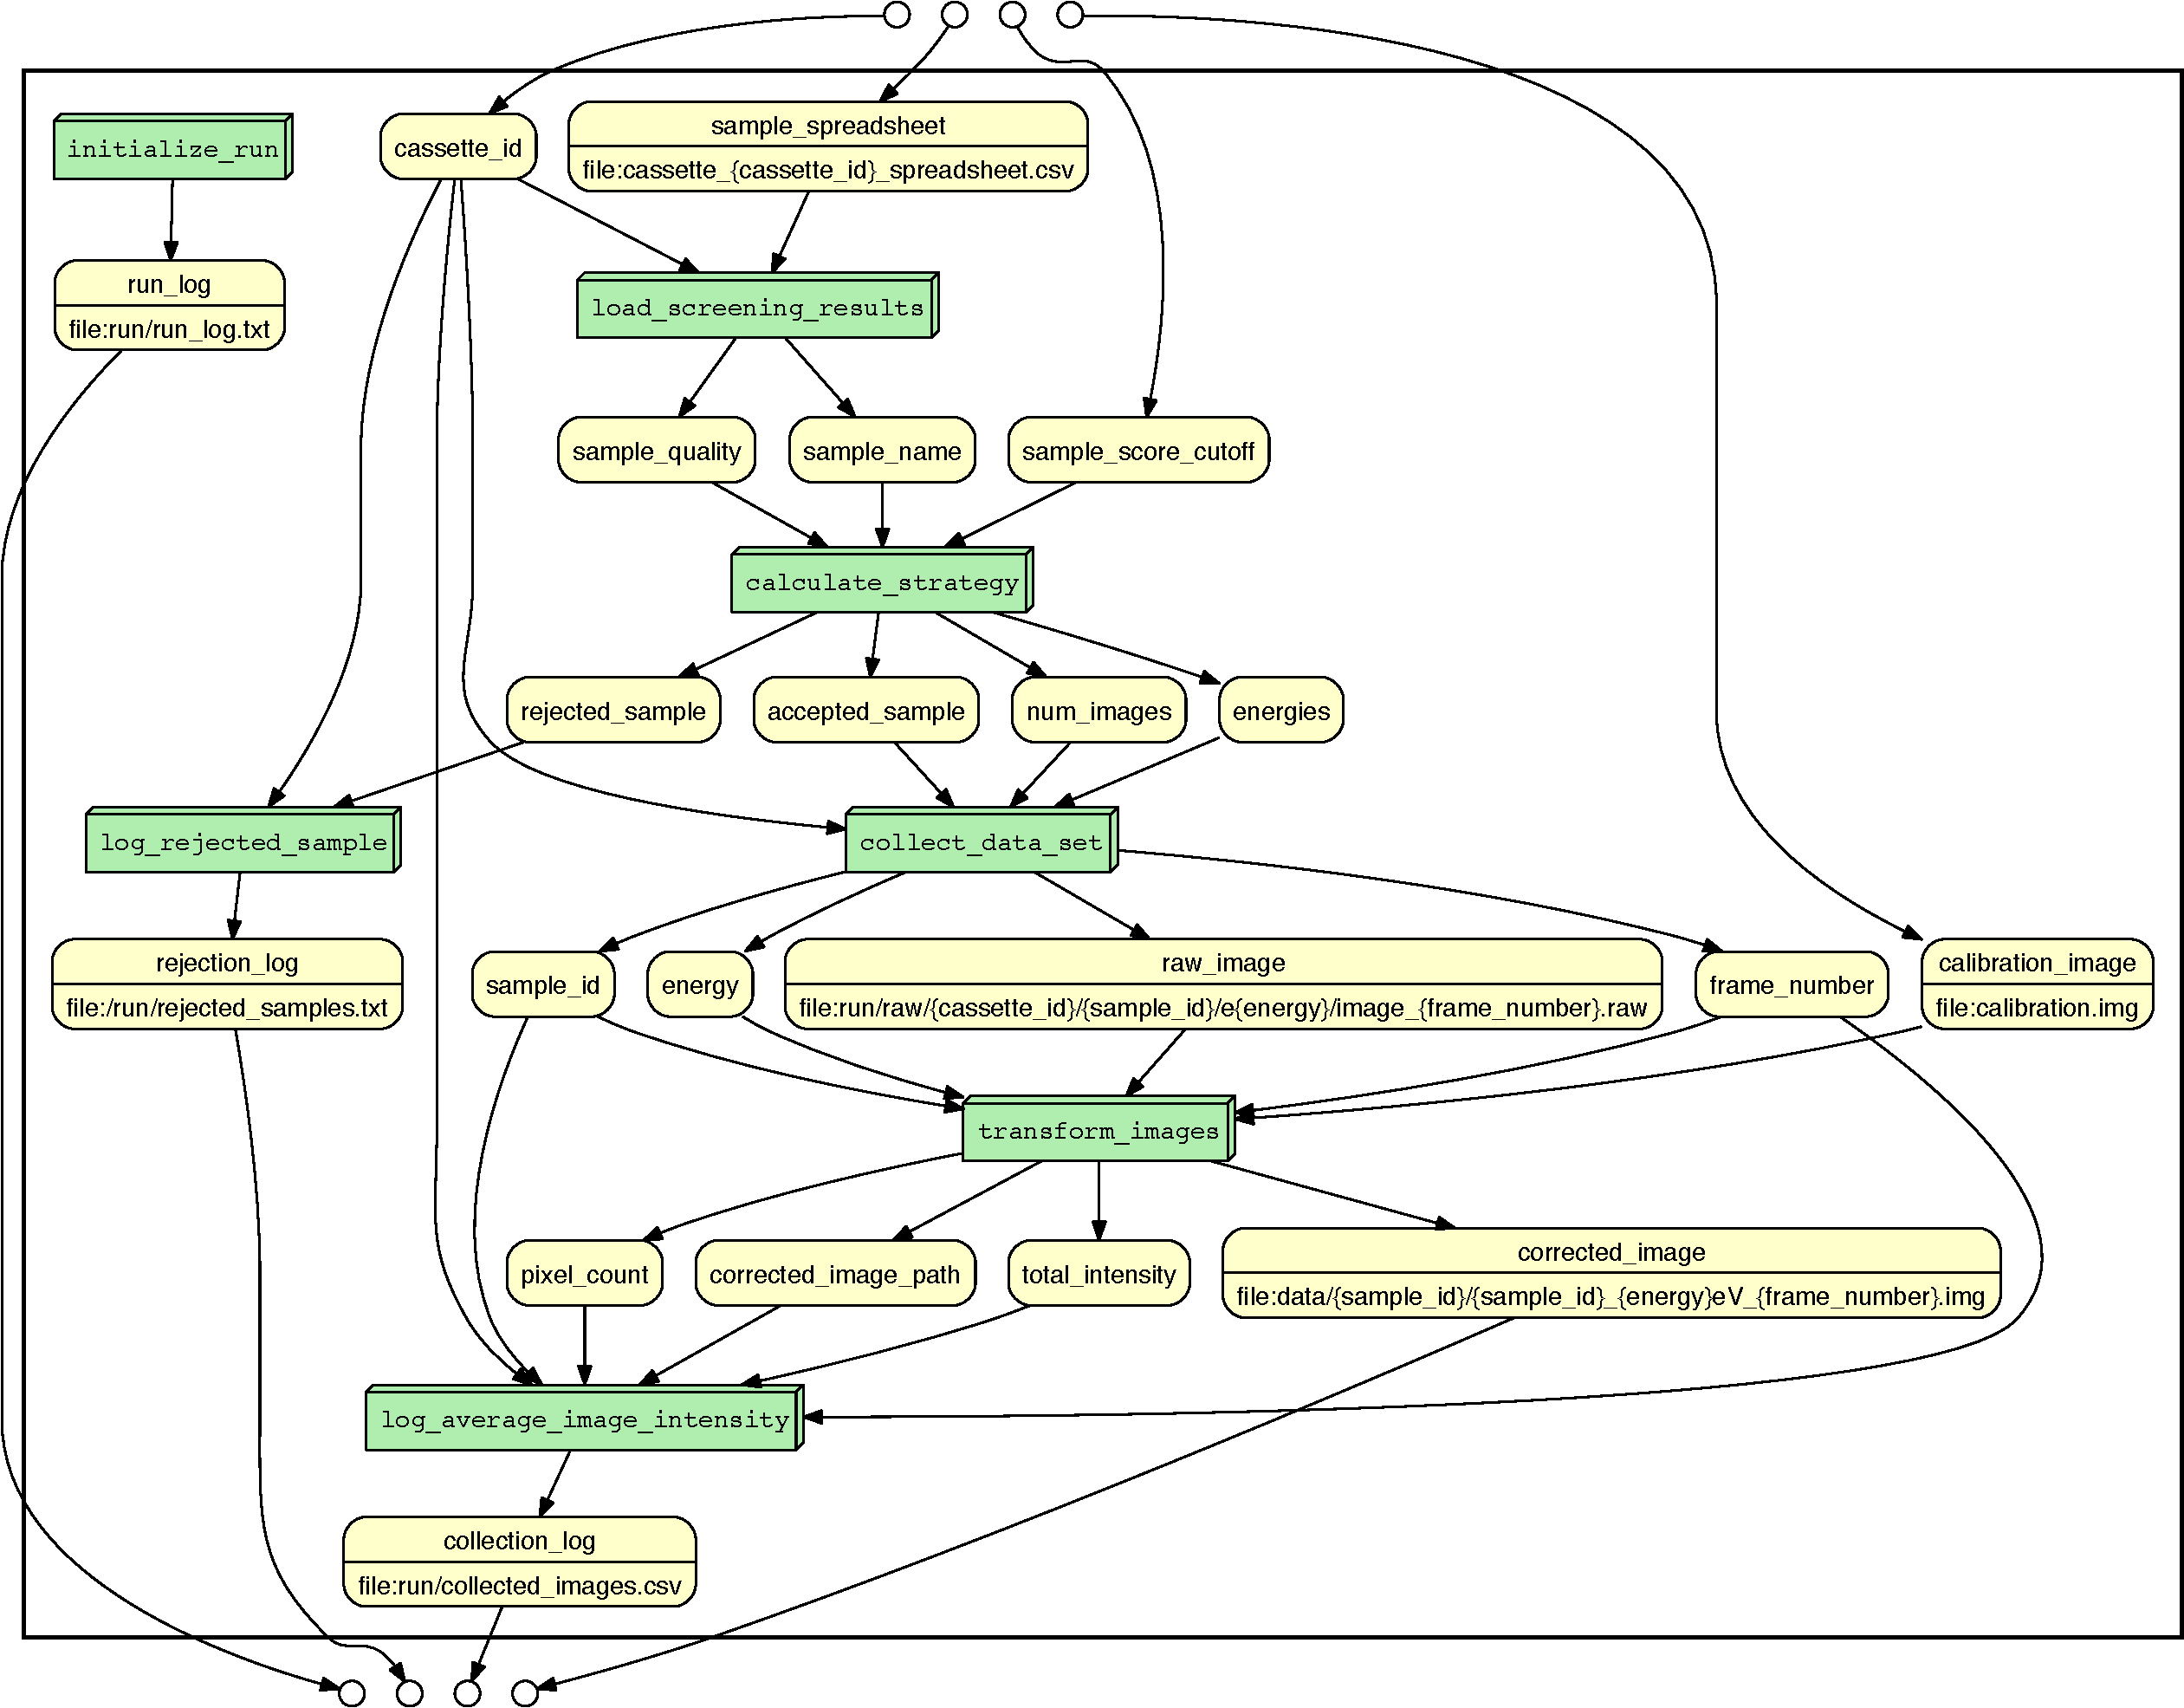
\includegraphics[width=.8\textwidth]{combined-crop.pdf}
  \caption{\small Workflow graph generated from \yw-annotations of the
    data collection script \cite{mcphillips2015example}.  Green boxes
    represent program blocks annotated in the Python script, while
    yellow rounded nodes represent data elements that flow between
    blocks.  Available URI templates are 
    depicted in the lower halves of data element nodes in
    the graph and specify the directory structure and file names for
    persisting those data. }
  \label{fig-wfgraph}
\end{figure*}


The script loads previously measured data quality statistics for each
sample (in \Figref{fig-wfgraph}, see the block
\code{load\_screening\_results}) from an input spreadsheet file
associated with the sample cassette used to store and transport the
samples; rejects samples that do not meet a minimum quality criterion;
and calculates an optimal data collection strategy
(\code{calculate\_strategy}) for each accepted sample (a data
collection strategy here comprises a set of data collection energies
and a count of diffraction images to collect at each energy). The
script then collects a series of diffraction images for each accepted
sample in turn, saving each raw detector image to the filesystem
(\code{collect\_data\_set}). The raw images are organized by sample
cassette ID, sample name, and X-ray beam energy; images in a sequence
collected on the same sample at the same energy are distinguished by a
frame number. A subsequent step transforms each raw image to a
corrected image using a detector-specific calibration image and saves
the resulting corrected images in a different set of output files and
directories (\code{transform\_images}).

\begin{figure}[thb]
  \centering
  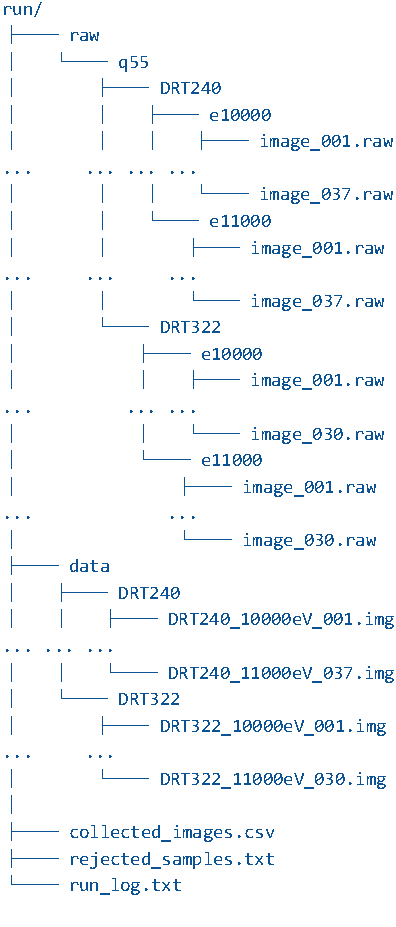
\includegraphics[width=.3\textwidth]{tree-abbrev-crop.pdf}
  \caption{\small Tree view of the directories and files created by
    the data collection Python script.}
  \label{fig-data-tree}
\end{figure}


% \section{Querying Retrospective Provenance} 
% \label{sec:queries}

% Our approach to revealing the retrospective provenance of script
% products in the absence of a provenance recorder is based on a number
% of observations. Many scientists use directory structures and
% directory and file names to organize data produced by scripts and to
% denote their relationships. In particular, when scientists write
% scripts they often have a set of retrospective provenance queries in
% mind that are of such high priority that they want to be able to
% answer them without interpreting the contents of log files. This is
% especially important when individual log files are independently
% written by different programs invoked by the single script.  The
% information required to answer these queries is therefore embedded by
% scientists in filenames, directory names, and in the hierarchical
% directory structures in which data is organized.  Our response to
% these observations is to let script writers describe this information
% naturally via URI template expressions. In this way \YW\ allows script
% writers to declare how script inputs and outputs are named and
% organized based on actual data and metadata values occurring at
% runtime.

% % Although looking through directories to understand what a script did
% % can be more effective than looking through multiple log files,
% With \YW\ we aim to make scientists even more productive by
% eliminating the need to explore directory structures manually.  \yw\
% can implement the scientists' high-priority questions as
% \emph{provenance queries} using the declared URI template information.

% % \YW\ thus can provide value by using the declared URI templates in
% % scripts to answer scientists' high-priority queries without requiring
% % them to inspect the contents of directories.

% We report in this section a number of typical provenance queries that
% are expressed against our example script. For each query we begin by
% describing how a scientist would determine the answer by inspecting
% the names and organization of the files produced by the script. We
% then provide a more general approach to answering each query that does
% not depend on the exact directory structure and file naming
% conventions used in the script (while continuing to assume that
% sufficient information is recorded in such a manner that a scientist
% could answer the question by hand and in the absence of runtime
% provenance recording.) 
% % For the first queries we also summarize how
% % these can be implemented using logic rules and facts produced by the
% % \yw\ tools.
% %  based on its analysis of the script and files it
% % discovers matching the URI templates in the script.

% Queries $Q_1$ and $Q_2$ represent script run \emph{reports}, i.e.,
% they answer questions that the user may have about the samples used,
% experimental conditions employed, and results obtained by the script.
% Queries $Q_3$ and $Q_4$, on the other hand, are backward and forward
% lineage queries, respectively. $Q_3$ identifies an intermediate data
% product that a specific final product was derived from; $Q_4$
% determines if there are any intermediate products for which there are
% no corresponding final products (this is an example of a
% \emph{why-not} provenance query). $Q_5$ can be viewed as a data
% lineage query that reveals the \emph{physical} provenance of a sample
% (the identity of a cassette that stores a specific sample).

% \paragraph{($Q_1$) \emph{What samples did the run of the script
%   collect images from?}} 
% The scientist's solution is to look at the contents of the
% \code{run/raw/q55} directory (\figref{fig-data-tree}). The names of
% subdirectories are the names of the samples collected on.

% \textbf{General solution using \yw}: Assume that `what samples' means
% `what values of \code{sample\_id} as seen by
% \code{collect\_data\_set}'. Then the solution is to look for all
% persisted outputs of \code{collect\_data\_set} that include
% \code{sample\_id} in the expanded URI template.
% Extract the value of \code{sample\_id} from each and return the set of
% unique values. $Q_1$ can be expressed as a Datalog query:
% \begin{verbatim}
% samples_used(SampleId) :- 
%     uri_variable_value(collect_data_set,
%                        raw_image_path,
%                        sample_id, 
%                        SampleId).
% \end{verbatim}
% against the provenance facts reconstructed by \yw. For our example, this will yield the
% answers \code{DRT240} and \code{DRT322}.


% \paragraph{($Q_2$): What energies were used during collection of
%   images from sample \code{DRT322}?}
% The scientist's solution is to look at the contents of the
% \code{run/raw/q55/DRT322} directory. The names of subdirectories are
% the values of the energies.

% \textbf{General solution using \yw}: Assume that `what energies' and
% `from sample \code{DRT322}' mean `what values of energy as seen by
% \code{collect\_data\_set} when \code{sample\_id} equals \code{DRT322}
% as seen by \code{collect\_data\_set}'.  Then the solution is to look
% for all persisted outputs of \code{collect\_data\_set} that include
% both energy and \code{sample\_id} in the expanded URI template for the
% output.  Extract the value of energy from each such path for which
% \code{sample\_id} equals \code{DRT322} and return the set of unique
% values.

% \paragraph{($Q_3$)
%   Where is the raw image corresponding to corrected image
%   \code{DRT322\_11000ev\_028.img}?}
% The scientist's solution is to look at the image files nested within
% the \code{raw} directory.  Find the image file that contains the
% \code{"DRT322"}, \code{"11000"}, and \code{"028"} in the file access
% path.

% \textbf{General solution using \yw}: Assume that `raw image for
% corrected image' means `what file output by the port named
% \code{raw\_image} with values for URI template variables equal to the
% matching URI template expansion variables in the path to the file
% \code{DRT322\_11000ev\_028.img} output by the port named
% \code{corrected\_image}'.  Then the solution is to extract the URI
% template variable names and values from the path to
% \code{DRT322\_11000ev\_028.img} output by the port named
% \code{corrected\_image}, look at the paths for all files output by the
% \code{raw\_image} port, and return the file whose path includes
% template variables with names and values matching those for
% \code{DRT322\_11000ev\_028.img} (not all variables need be present in
% both paths, but where the variable with same name is used the values
% must match).

% \paragraph{($Q_4$)
%   Are there any raw images for which \emph{no} corrected image was written?}
% This is somewhat similar to $Q_ 3$, but follows the lineage in the
% ``forward direction'' and (unlike $Q_4$) asks about the absence of
% data.  In this case the path to each file written by the
% \code{raw\_image} port is examined, and a corresponding file written
% by the \code{corrected\_image} port is sought.  Return raw images for
% which no corrected image is found.

% \paragraph{($Q_5$) What was the id of the cassette from which sample
%   leading to \code{DRT240\_10000ev\_010.img} was taken?} This query
% shows how the retrospective data lineage information can be used to
% track the physical provenance of samples.  The general solution here
% is to search the upstream lineage of data provided to
% \code{transform\_images}, looking for URI templates that include
% \code{cassette\_id} and \code{sample\_id} as template
% variables. Return the value of \code{cassette\_id} that occurs in URI
% expansions where \code{sample\_id} matches \code{DRT240}.

% \paragraph{Example Code.}
% The example Python code, along with the \yw-generated prospective
% provenance shown in \figref{fig-wfgraph}, and some of the
% \yw-reconstructed retrospective provenance facts and rules are
% available from \cite{mcphillips2015example}.


\section{Querying Retrospective Provenance} 
\label{sec:queries}

Our approach to revealing the retrospective provenance of script
products in the absence of a provenance recorder is based on a number
of observations. Many scientists use directory structures and
directory and file names to organize data produced by scripts and to
denote their relationships. In particular, when scientists write
scripts they often have a set of retrospective provenance queries in
mind that are of such high priority that they want to be able to
answer them without interpreting the contents of log files. This is
especially important when individual log files are independently
written by different programs invoked by the single script.  The
information required to answer these queries is therefore embedded by
scientists in filenames, directory names, and in the hierarchical
directory structures in which data is organized.  Our response to
these observations is to let script writers describe this information
naturally via URI template expressions. In this way \YW\ allows script
writers to declare how script inputs and outputs are named and
organized based on actual data and metadata values occurring at
runtime.

% Although looking through directories to understand what a script did
% can be more effective than looking through multiple log files,
With \YW\ we aim to make scientists even more productive by
eliminating the need to explore directory structures manually.  \yw\
can implement the scientists' high-priority questions as
\emph{provenance queries} using the declared URI template information
together with dependencies introduced by \YW\ script annotations.

% \YW\ thus can provide value by using the declared URI templates in
% scripts to answer scientists' high-priority queries without requiring
% them to inspect the contents of directories.

We report in this section a number of typical provenance queries that
are expressed against our example script. For each query we begin by
describing how a scientist would determine the answer by inspecting
the names and organization of the files produced by the script. We
then provide a more general approach to answering each query that does
not depend on the exact directory structure and file naming
conventions used in the script (while continuing to assume that
sufficient information is recorded in such a manner that a scientist
could answer the question by hand and in the absence of runtime
provenance recording.)

% For the first queries we also summarize how
% these can be implemented using logic rules and facts produced by the
% \yw\ tools.
%  based on its analysis of the script and files it
% discovers matching the URI templates in the script.

Queries $Q_1$ and $Q_2$ represent script run \emph{reports}, i.e.,
they answer questions that the user may have about the samples used,
experimental conditions employed, and results obtained by the script.
Queries $Q_3$ and $Q_4$, on the other hand, are backward and forward
lineage queries, respectively. $Q_3$ identifies an intermediate data
product that a specific final product was derived from; $Q_4$
determines if there are any intermediate products for which there are
no corresponding final products (this is an example of a
\emph{why-not} provenance query). $Q_5$ can be viewed as a data
lineage query that reveals the \emph{physical} provenance of a sample
(the identity of a cassette that stores a specific sample).

As shown below, these and similar queries are answered by generating a
set of relations corresponding to a script's workflow (as defined by
\YW\ annotations) as well as information about resources and their
metadata attributes (from the files generated by a run of the script
and the corresponding URI template information). The result of this
\emph{provenance reconstruction} process generates the base relations
shown in Table~\ref{tbl:baserels}.

%%%%%%%%%%%%%%%%%%%%%%%%%%%%%%%%%%%%%%%%%%%%%%%%%%%%%%%%%%%%%%%%%%%%%%
\begin{table*}[!t]
\nocaptionrule
\caption{Base relations generated by the \YW\ provenance 
  reconstruction process.}
\label{tbl:baserels}
\begin{footnotesize}
\begin{tabular}{|l|l|} \hline
{\em Base Relation} & {\em Description} \\ \hline\hline

{\tt program(}{\em id,name,begin\_annot,end\_annot}{\tt )} & 
Identifier, name, and annotation start and end line of workflow 
program blocks
\\ \hline

{\tt port(}{\em id,type,name,annot\_id}{\tt )} & 
Identifier, type (in, out, param), name, and annotation identifier
of workflow ports
\\ \hline

{\tt port\_alias(}{\em port\_id,alias\_name}{\tt )} &
Alias names given to ports (specified via {\tt @AS} annotations) 
\\ \hline

{\tt has\_in\_port(}{\em program\_id,port\_id}{\tt )} &
Input ports of program blocks 
\\ \hline

{\tt has\_out\_port(}{\em program\_id,port\_id}{\tt )} &
Output ports of program blocks 
\\ \hline

{\tt channel(}{\em id,binding}{\tt )} & 
Assignment of script variables to channels
\\ \hline

{\tt port\_connects\_to\_channel(}{\em port\_id,channel\_id}{\tt
    )} & 
Assignment of ports to channels 
\\ \hline

{\tt uri\_variable(}{\em id,name,port\_id}{\tt )} & 
Identifier, name, and associated port of URI metadata variables 
\\ \hline

{\tt resource(}{\em id,uri}{\tt )} & 
Identifier and expanded URI (file path) of resources created by a run of the script 
\\ \hline

{\tt resource\_channel(}{\em resource\_id,channel\_id}{\tt )} & 
Resources that were input to or output by a channel
during a run of the script
\\ \hline  

\end{tabular}
\end{footnotesize}
\end{table*}
%%%%%%%%%%%%%%%%%%%%%%%%%%%%%%%%%%%%%%%%%%%%%%%%%%%%%%%%%%%%%%%%%%%%%%


\paragraph{($Q_1$) \emph{What samples did the run of the script
  collect images from?}} 
The scientist's solution is to look at the contents of the
\code{run/raw/q55} directory (\figref{fig-data-tree}). The names of
subdirectories are the names of the samples collected on.

\textbf{General solution using \yw}: Assume that `what samples' means
`what values of \code{sample\_id} as seen by
\code{collect\_data\_set}'. Then the solution is to look for all
persisted outputs of \code{collect\_data\_set} that include
\code{sample\_id} in the expanded URI template.
Extract the value of \code{sample\_id} from each and return the set of
unique values. $Q_1$ can be expressed as the Datalog query:
\begin{small}
\begin{verbatim}
samples_used(SampleId) :- 
   resource_info(ResourceId,collect_data_set,
                 raw_image,sample_id,SampleId).
\end{verbatim}
\end{small}
where {\tt resource\_info} is a simple view expressed against the
provenance facts reconstructed by \yw\ to obtain the program, port
name, and metadata information of resources.  For our example, the
above query will yield the answers \code{DRT240} and \code{DRT322}.


\paragraph{($Q_2$): What energies were used during collection of
  images from sample \code{DRT322}?}
The scientist's solution is to look at the contents of the
\code{run/raw/q55/DRT322} directory. The names of subdirectories are
the values of the energies.

\textbf{General solution using \yw}: Assume that `what energies' and
`from sample \code{DRT322}' mean `what values of energy as seen by
\code{collect\_data\_set} when \code{sample\_id} equals \code{DRT322}
as seen by \code{collect\_data\_set}'.  Then the solution is to look
for all persisted outputs of \code{collect\_data\_set} that include
both energy and \code{sample\_id} in the expanded URI template for the
output.  Extract the value of energy from each such path for which
\code{sample\_id} equals \code{DRT322} and return the set of unique
values. $Q_2$ can be expressed as the Datalog query: 
\begin{small}
\begin{verbatim}
energies_used(EnergyValue) :-
   resource_info(ResourceId,collect_data_set,
                 raw_image,sample_id,"DRT322"),
   resource_info(ResourceId,collect_data_set,
                 raw_image,energy,EnergyValue).
\end{verbatim}
\end{small}
For our example, the above query will yield the answers \code{10000}
and \code{11000}.

\paragraph{($Q_3$)
  Where is the raw image corresponding to corrected image
  \code{DRT322\_11000ev\_028.img}?}
The scientist's solution is to look at the image files nested within
the \code{raw} directory.  Find the image file that contains the
\code{"DRT322"}, \code{"11000"}, and \code{"028"} in the file access
path.

\textbf{General solution using \yw}: Assume that `raw image for
corrected image' means `what file output by the port named
\code{raw\_image} with values for URI template variables equal to the
matching URI template expansion variables in the path to the file
\code{DRT322\_11000ev\_028.img} output by the port named
\code{corrected\_image}'.  Then the solution is to extract the URI
template variable names and values from the path to
\code{DRT322\_11000ev\_028.img} output by the port named
\code{corrected\_image}, look at the paths for all files output by the
\code{raw\_image} port, and return the file whose path includes
template variables with names and values matching those for
\code{DRT322\_11000ev\_028.img} (not all variables need be present in
both paths, but where the variable with same name is used the values
must match).  $Q_3$ can be expressed as the Datalog query: 
\begin{small}
\begin{verbatim}
raw_image_used(RawImageFile) :-
   resource(CorrectedImage,"./run/data/
            DRT322/DRT322_11000eV_028.img"),
   channel(RawImageChannel,raw_image),
   resource_channel(RawImage,RawImageChannel),
   depends_on(CorrectedImage,RawImage),
   resource(RawImage,RawImageFile).
\end{verbatim}
\end{small}
This query relies on a {\tt depends\_on} relation that computes the
dependencies between resources based on their metadata values and the
workflow graph. In particular, a resource $r_2$ is presumed to have
depended on a resource $r_1$ if: (i) $r_1$ is upstream of $r_2$ in the
corresponding \YW\ workflow graph (based on input-output ports and
channels defined in the script); (ii) $r_1$ and $r_2$ have at least
one metadata variable in common (based on their corresponding URI
templates); and (iii) the metadata variables in common between $r_1$
and $r_2$ have the same values for $r_1$ and $r_2$ (based on their
expanded URIs). \Figref{fig:depends-on} gives a definition of the {\tt
  depends\_on} relation as a Datalog program.

\begin{figure*}[!t]
  \begin{footnotesize}
  \begin{verbatim}
                   depends_on(R1,R2) :- upstream_resource(R2,R1), R1!=R2, common_metadata_var(R1,R2), 
                                        not common_metadata_values_differ(R1,R2), 
          common_metadata_var(R1,R2) :- uri_resource_var_value(R1,N,_), uri_resource_var_value(R2,N,_).
common_metadata_values_differ(R1,R2) :- resource_channel(R1,C1), resource_channel(R2,C2), 
                                        uri_resource_var_value(R1,N,V1), 
                                        uri_resource_var_value(R2,N,V2), V1!=V2.
       uri_resource_var_value(R,N,V) :- uri_variable(X,N,_), uri_variable_value(R,X,V).
            upstream_resource(R1,R2) :- resource_channel(R1,C1), port_connects_to_channel(P1,C1), 
                                        resource_channel(R2,C2), port_connects_to_channel(P2,C2), 
                                        port_dep_tc(P2,P1).
                     port_dep(P2,P1) :- has_in_port(B,P1), has_out_port(B,P2).
                     port_dep(P2,P1) :- has_in_port(_,P2), has_out_port(_,P1), channel(C,_), 
                                        port_connects_to_channel(P1,C), port_connects_to_channel(P2,C).
                  port_dep_tc(P2,P1) :- port_dep(P2,P1).
                  port_dep_tc(P2,P1) :- port_dep_tc(P2,P), port_dep_tc(P,P1).
  \end{verbatim}
  \end{footnotesize}
  \caption{A Datalog program for calculating resource dependencies ({\tt depends\_on}) in \YW.}
  \label{fig:depends-on}
\end{figure*}

\paragraph{($Q_4$)
  Are there any raw images for which \emph{no} corrected image was written?}
This is somewhat similar to $Q_ 3$, but follows the lineage in the
``forward direction'' and (unlike $Q_4$) asks about the absence of
data.  In this case the path to each file written by the
\code{raw\_image} port is examined, and a corresponding file written
by the \code{corrected\_image} port is sought.  Return raw images for
which no corrected image is found. $Q_4$ can be expressed as the Datalog query:

\begin{small}
\begin{verbatim}
no_corrected_image_written(RawImageFile) :-
   channel(RawImageChannel,raw_image),
   resource_channel(RawImage,RawImageChannel),
   not corrected_raw_image(RawImage),
   resource(RawImage,RawImageFile).

corrected_raw_image(RawImage) :-
    channel(RawImageChannel,raw_image),
    resource_channel(RawImage,RawImageChannel),
    channel(CorrectedImageChannel,corrected_image),
    resource_channel(CorrectedImage,
                     CorrectedImageChannel),
    depends_on(CorrectedImage,RawImage).
\end{verbatim}
\end{small}
In this case, the {\tt corrected\_raw\_image} relation finds those raw
images that do have a corresponding corrected image written. To answer
the query, we find exactly those raw images for which {\tt
  corrected\_raw\_image} fails (thus implying the raw image has no
corrected image).

\paragraph{($Q_5$) What was the id of the cassette from which the
  sample leading to \code{DRT240\_10000eV\_010.img} was taken?} This
query shows how the retrospective data lineage information can be used
to track the physical provenance of samples.  The general solution
here is to search the upstream lineage of data provided to
\code{transform\_images}, looking for URI templates that include
\code{cassette\_id} and \code{sample\_id} as template
variables. Return the value of \code{cassette\_id} that occurs in URI
expansions where \code{sample\_id} matches \code{DRT240}. $Q_5$ can be
expressed as the Datalog query:
\begin{small}
\begin{verbatim}
cassette_used(CassetteId) :-
   resource(CorrectedImage,"./run/data/
            DRT240/DRT240_10000eV_010.img"),
   program(TransformImages,transform_images,_,_),
   has_in_port(TransformImages,InPort), 
   port_connects_to_channel(InPort,Channel), 
   resource_channel(Resource,Channel), 
   depends_on(CorrectedImage,Resource), 
   uri_resource_var_value(Resource,cassette_id,
                          CassetteId).
\end{verbatim}
\end{small}
For our example, the above query will yield the cassette id ``q55''. 

\paragraph{Example Code.}
The example Python code, along with the \yw-generated prospective
provenance shown in \figref{fig-wfgraph}, and some of the
\yw-reconstructed retrospective provenance facts and rules are
available from \cite{mcphillips2015example}.


%%% Local Variables:
%%% mode: latex
%%% TeX-master: "yw-prov-recon"
%%% End:



\section{Discussion and Conclusions} 
\label{sec:discussion}

The idea of using prospective and retrospective provenance for a wide
range of applications is not new (see, e.g.,
\cite{zhao2006applying,missier2008data,frew2008automatic}).  It is
widely known that by employing scientific workflow systems, users can
benefit from prospective provenance (through workflow descriptions)
and retrospective provenance (from runtime provenance recording)
information. On the other hand, it is much less well known that an
annotation-based approach such as \YW\ can be used to obtain
prospective provenance and---as illustrated in this
paper---retrospective provenance as well, without the use of a runtime
provenance recorder.  We have implemented and continue to improve the
\yw\ toolkit \cite{mcphillips2015ywIJDC,yw-website}. Using simple
\yw-annotations, a scientist can use our toolkit to easily and
quickly\footnote{The first author of \cite{bocinsky2014} reported that
  creating the annotations for the \yw-model depicted in
  \cite{mcphillips2015ywIJDC} (for an \R\ script used in
  \cite{bocinsky2014}) took only half an hour.}  create a high-level
dataflow model for a script-based workflow.  Since \yw-annotations are
embedded as comments in the host language, our approach is
language-independent, and can be applied to any of the usual scripting
or programming languages.

In this paper, we also have shown that retrospective provenance from
scripts can be easily obtained and combined with prospective
provenance using new \yw-annotations with URI templates. For this
simple approach to work, we make the (realistic) assumption that
scientists organize their data using directories for staging and
collecting data files: e.g., Bowers \emph{et al.}
\cite{bowers2007project} includes a detailed account of how a
metagenomics researcher organizes his data and results in a nested
folder scheme. Moreover, the URI template approach for declaring the
layout of data persisted by a workflow run in nested directories has
been employed by the RestFlow scientific workflow system
\cite{tsai2013autodrug}.
% , where it is used by the workflow designer to
% declare how workflow products should be organized by the system.
Despite being a grass-roots effort that was launched only recently,
\yw\ has already been successfully applied to real-world, script-based
workflows in \R, \MATLAB, and Python; application domains include
climate modeling, bioinformatics, and archeology
\cite{mcphillips2015ywIJDC}.
In future work, we will explore other community efforts to workflow
modeling such as the Common Workflow Language \cite{amstutz15CDL} and
the Workflow Description Language \cite{frazer15WDL} for use in \YW.

\paragraph{Acknowledgments.}
Work supported in part by the National Science Foundation under awards
DBI-1356751 (Kurator), SMA-1439603 (SKOPE), ACI-0830944 (DataONE).


\bibliographystyle{alpha-initials-big}
\footnotesize
\bibliography{yw-prov-recon}



\end{document}







